% (c) 2020 Stefan Antonowicz
% Based off of tex found at https://github.com/ludus-leonis/nipajin
% This file is released under Creative Commons Attribution-NonCommercial-ShareAlike 4.0 International License.
% Please do not apply other licenses one-way.

\renewcommand{\yggArbiter}{%
  \mychapter{Arbiter}{arbiter}
}

\renewcommand{\yggArbiterText}{%

  \mysection{Miscellania}{arbiter-miscellania}

  \mysubsection{Adding and Splitting Usage Dice}{arbiter-miscellania-splitting-ud}

  To avoid mathematical insanity, \UD can only be a) combined with another UD of the same type or b) split into 2 equal \UD.  You can't split a d4 \UD, and you can't combine a d20 or d24 \UD

  \mytable{X c c}{
    \thead{\UD} & \thead{Combine Into...} & \thead{Split Into ...} \\
  }{
    d2 & d3 & n/a \\
    d3 & d4 & n/a \\
    d4 & d6 & n/a \\
    d6 & d10 & 2 d4 \\  
    d8 & d12 & 2 d6 \\
    d10 & d16 & 1 d6 + 1 d8 \\
    d12 & d20 & 2 d8 \\
    d16 & d24 & 2 d10 \\
    d20 & n/a &  2 d12 \\
    d24 & n/a & 2 d16 \\
  }


  \mysection{Movement}{arbiter-movement}


  \mysubsection{Getting Chased}{arbiter-movement-getting-chased}

  Both the pursuer and the pursued roll an \RB : \MD.  Unless they split up, use the lowest \MD in the group.

  The loser moves their \MD \DCDOWN, the winner moves their \MD is \DCUP (track this separately, this is just for the purposes of the chase).  The chase ends when someone loses on a d4 or wins on a d20.  During a chase, any Shoot or Throw attacks suffer a penalty equal to the opponent's \MAX \MD (-4 for a d4, -8 for a d8, etc)

  If someone is being chased and the pursuer rolls a Failure on their \MD, the adventurer being chased can try to do something to lose them (so in a city something like jumping onto a roof or into an alley or a random doorway or spilling a cart in front of them). If they win the next check, they lose the pursuer and the chase is over.

  If a adventurer is pursuing someone and their prey rolls a Failure on their \MD, the adventurer can try to do something to stop them (like yelling at Old Bob who's always standing in front of the Bloated Cuttlefish to grab them).  If they win the next check, they catch their prey and the chase is over.


  \mysubsection{Jumping Distances}{arbiter-movement-jumping}

  If an adventurer is trying to jump over something, they must \RO using their \MD plus either \VIG or \DEX (their choice) plus a modifier for distance:

  \example {
    \RO : \MD plus \VIG or \DEX plus Modifiers
  }

  The modifier depends on whether or not they have a running start. A adventurer can't jump more than 9m (4m if standing):

  \mytable{c c c}{
    \thead{Distance(m)} & \thead{Running Bonus} & \thead{Standing Bonus} \\
  }{
    1 & +9 & -3 \\
    2 & +7 & -5 \\
    3 & +5 & -7 \\
    4 & +3 & -9 \\  
    5 & +0 & n/a \\
    6 & -3 & n/a \\
    7 & -5 & n/a \\
    8 & -7 & n/a \\
    9 & -9 & n/a \\
  }

  \example {
    An unarmored person (d20) with a d12 \DEX wants to make a running jump over a 3m pit.  They have to \RO with a d20+d12+5 (about a 63\% chance)
    ~\\
    The Solider with Heavy armor (d4) and a d16 \VIG would need to \RO with a d20+d4+5 to jump over the same pit (about a 43\% chance).
  }

  \mysubsection{Climbing and Falling}{arbiter-movement-falling}
  There's no damage if you fall 5m or less.  

  For every meter over 5 you fall, you take 1 damage (so 6m would be 6 damage).  This damage can be absorbed by Armor but not Grit (or a shield).  

  You get 2 chances to reduce damage:
  \mynumlist {
    \item Roll a \RS : Talent. If you succeed,  take half damage (if you fail, move your \UD \DCDOWN)
    \item Make a Save vs. Doom.  If you succeed, take half damage again.
  }

  These effects stack - so making your Talent roll + Save vs. Doom will reduce the amount of damage by 75\%.  Roll the check and Save before you apply damage to Armor or Flesh.  If falling means you are \mylink{Dying}{combat-dying}, you also take the effects of \mylink{Bleeding}{effect-bleeding} and \mylink{Knocked Out}{effect-knocked-out}



\mysubsection{Swimming}{arbiter-movement-swimming}

Swimming is fairly straightforward:

\mybullet {
    \item   If the adventurer is in Combat, all Actions take twice as long i.e.  it will take them two Maneuvers to move from Close to Nearby, two Maneuvers to get something from their pack, etc.
    \item   The adventurer is unable to Fight or Guard while swimming
    \item   The adventurer cannot be carrying any Significant Items
}

Adventurers are heroic, so they should generally be able to swim long distances without any additional checks.  However, in high seas or over very long distances, the Arbiter can have the advenuturer attempt a Skill:Salt check.  If they fail, they begin drowning unless they can breathe underwater.  Each time they fail their Skill:Salt roll, they must make a \DEATH roll.  Each time they fail thereafter, they receive a -2 cumulative modifier (-2 the first time, -4 the second, -6 the third, etc).  

  \myhighlight{Removing Armor}{gear-armor-removal} 

  Helmets, Shields, and Light Armor take Moments to remove.  Medium and Heavy Armor take Minutes to remove.

\cbreak

  \mysubsection{Random Encounters}{arbiter-movement-random-encounters}

  The lowest \MD in the party is used for random encounter checks using a \RS : \MD.  Failure means a wandering Monster shows up. 

  \mysubsection{Dangerous Terrain}{arbiter-movement-dangerous-terrain}

  If the adventurers are crossing an area that is dangerous, or where time is of the essence, give the room a total number that you need to roll to cross it.  Every \MD roll takes a Moment - so crossing the room with a movement number of 12 will require at least 3 Moments for the adventurer in Heavy Plate (3d4), while the guy in a nightshirt has a 45\% to do it in one shot.


  \begin{center}
  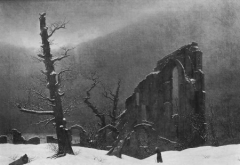
\includegraphics{Ruins}
  \end{center}

 

 \end{multicols}


  \mysection{Knavery}{arbiter-knave}

   First - a \KNAVE roll should only be required if the difference between success and failure would be interesting, or when the attempt shouldn't be an automatic success.  If either of these cases are true, let the Knave succeed without rolling anything.

  Setting a difficulty for a Knave's \mylink{Whisper}{knave-whispers} abilities means picking a number between 2 and 9 (remember the Adventurer can only add a \MAX of +4 to their \KNAVE roll with their Luck).



  \begin{multicols}{2}
  \raggedcolumns
  \mybold{\mylink{Whispers of Anne Bonny}{knave-virtue-ann-bonny}}

  \mybold{Climbing:} Every 10m should be a point of difficulty.  Add a point if the wall is particularly slippery, it's windy, or if the Knave is encumbered or injured; subtract a point if the Knave has rope or climbing gear, or strips off equipment to make climbing easier.

   \mybold{Disguise and Forgery:}   Using minor details to disguise yourself as a stranger, or lying to a kid might be a 2; changing your gender or species, or forging an arrest warrant, might be a 4 or 5; pretending you're someone famous might be a 7; lying to a Sphinx, forging an Article of War, or fooling a close friend might be a 9.


    \mybold{\mylink{Whispers of Br'er Rabbit}{knave-virtue-brer-rabbit}}

    \mybold{Picking Pockets:} Picking the pocket of a common yokel in a crowded street might be a 2; stealing the keys from a guard's belt might be a 5; palming a card in a game with demons might be a 7; stealing the rings from the king's finger when you kiss his hand might be a 9.



    \mybold{\mylink{Whispers of Sun Wukong}{knave-virtue-sun-wukong}}

      \mybold{Locks:} A common lock on a blacksmith's shop might be a 2; your hands bound with rope might be a 4; a jeweller's lockbox in a Large settlement might be a 5; slipping free of manacles might be a 6;  an item locked by the Lock spell might be a 7; the lock on the Gates of Hell would be a 9.

       \mybold{Traps:} assign two difficulties - the difficulty of \mybold{finding} the trap and the difficulty of \mybold{disarming} a trap.  A hunter's snare or goblin trap might be a 2 or 3; a elaborate Rube Goldeberg trap in a mummy's tomb might be a 5; an invisible tripwire that triggers an explosion might be a 7; a trap designed by an Grimtooth might be a 9.

      Inscribed Sigils\footnote{See Bell, Book, and Candle} can also be disarmed with the Whispers of Sun Wukong. Iron Sigils are a 3, Silver Sigils are a 6, and Primary Sigils are a 9.


    \mybold{\mylink{Whispers of The Bride}{knave-virtue-the-bride}}
  
    \mybold{Sneaking:} Assign a point of difficulty for each \HD of a Monster.  Add a point if the area is well lit; add another point if the Knave is trying to slip past guards or someone looking for them.  Subtract a point for dark areas or distractions.

    A crowded room or shadowy street might be a 2 or 3; through a guarded doorway lit by torches might be a 6; hiding in someone's shadow in a well lit room might be a 9.


\mysection{Travel}{arbiter-travel}

\ed{This idea is taken from John Carr's \href{https://ageofruins.wordpress.com/2012/10/18/deck-of-many-threats-wilderness-encounters-based-on-playing-cards-plus-a-simple-system-for-provisions/}{Age of Ruins}}

\mysubsection{Journeys}{arbiter-travel-journeys}
Journeys consist of a number of routes (called Legs) to get from one point to another.  These routes are sometimes defined ("the Iron Road", "the High Pass", etc.) but the adventurers will often make routes of their own from looking at a map.  For example, "we must bear north, following the Miskatonic River, until we reach the mouth of the bay.  From there we will follow the coast west until we reach the point where the Iron Road meets Portsmouth, then follow the road south to Erl" is a journey of 3 legs (north to the bay, west to the road, south to Erl).

To figure out what happens on a Journey, you'll need a deck of cards.  Leave the Jokers in.

\mysubsection{Legs}{arbiter-travel-legs}
Roughly speaking, each leg of a journey is about 5-10 Days (50-100 leagues) (this can change at the Arbiter's discretion).  The Arbiter should assign a Danger value to each leg on a scale of 1 (the Gold Road) to 6 (trog-infested swamps).  The Arbiter should inform the adventurers of the Danger value of each Leg before they set out, in case they want to change their mind.

Grab a deck of cards.  For each Leg, draw a number of cards equal to the Danger of the Leg.  You'll use the same deck of cards for the entire Journey (so don't shuffle the cards back in until the Journey is complete).

If you don't draw a face card, an Ace, or a Joker - nothing happens.  If you do, first check the suit :

  \mytable{X c}{
    \thead{Suit} & \thead{Effect} \\
  }{
    \mybold{Clubs} & Roll your Party Provisions \UD \\
    \mybold{Diamonds} & You hit some bad weather  \\
    \mybold{Hearts} & You get lost or are off course \\
    \mybold{Spades} & You run into some hostiles  \\
    \mybold{Jokers} & You stumble on something interesting ... \\
  }

  Next, check the type of card to see when the event takes place:


  \mytable{X c}{
    \thead{Face} & \thead{Effect} \\
  }{
    \mybold{Jack} & Predawn \\
    \mybold{Queen} & Morning  \\
    \mybold{King} & Afternoon \\
    \mybold{Ace} & Evening  \\
    \mybold{Joker} & Arbiter's Choice \\
  }     


  \mysubsection{Party Provisions}{arbiter-travel-provisions}
  Roll your Party Provisions if you pull a Club (rats ate the flour; the mule stumbled and dropped the bacon in a river; etc) and at the end of a Leg of your Journey.  Before this roll, someone in your party must roll their Skill: Travel.  If they succeed, the Provisions \UD only drops \DCDOWN if you roll a 1 (instead of a 1 or 2).  

  \mysubsection{Bad Weather}{arbiter-travel-weather}
  You hit appropriate bad weather (snowstorm, sandstorm, torrential downpour, etc).  Someone in your party must roll their Skill: Travel.  If they succeed, nothing happens.  If they fail, roll a d3:  1) roll your Party Provisions, 2) you're Lost, 3) you run into Hostilities.


  \mysubsection{Lost}{arbiter-travel-lost}
  This can only happen if you are \myital{not} on a road. If you're traveling by road, you can ignore this result.

  Someone in your party must roll their Skill: Travel.  If they succeed, you get back on track.  If they fail, pull another card. The Arbiter will move you in a random direction (on a hex map, roll a d6 and move the party in that direction). Continue in this way until someone succeeds at their Skill: Travel roll.  


  \mysubsection{Hostiles}{arbiter-travel-hostiles}

  Roll on your random monster table for this area

  \mysubsection{Something Interesting}{arbiter-travel-pointofinterest}

  This can only happen if you are \myital{not} on a road. If you're traveling by road, ignore this result.  This is entirely up to the Arbiter, but might include : entrance to a small dungeon, weird shrine to a lost god, abandoned gnoll war camp, etc.


  \mysubsection{We're Out of Food}{arbiter-travel-starvation}
  If you run out of food, time switches to Game Time.  The Arbiter should determine how many Days the party is from their destination (the party can cover 10 leagues / 1 hex on a road every Day, whereas it might take 3 Days to cover 1 hex in the mountains).  The party should now follow the rules as if they were in a wilderness dungeon, including rolling Personal Provisions, using their Skill: Bushcraft, etc. 


  \newpage

\mysection{Monsters}{arbiter-monsters}


\mysubsection{Monster Morale}{monster-morale}

Morale is broken into 3 general types:  Cowardly, Orderly, and Fanatical.  Roll Morale by rolling 2d6 - if the number is greater than the basic roll (but not equal to!), they will attempt to flee or surrender.

\mybullet {
  \item \mybold{Cowardly} Basic roll is 3.  If the Monsters are in a group, roll a) when the first Monster dies (but only if the Monsters are outnumbered; b) when half the Monsters are down; or c) whenever a "leader" dies.  If the Monster is by itself, roll a) when it first takes damage and b) when it's at half Health or less.

  \item \mybold{Orderly} Basic roll is 7.  If the Monsters are in a group, roll a) when half the Monsters are down; or b) if \mybold{all}  the leaders are dead.  If the Monster is by itself, roll when it's at half Health or less.

  \item \mybold{Fanatical}  Basic roll is 11.  If the Monsters are in a group, roll when half the Monsters are down AND all the leaders are dead.  If the Monster is by itself, it will automatically pass a morale check.
}

\mysubsection{Monster Modifiers}{monster-modifiers}

\myhighlight{Monster Speed}{monster-speed}

  \mytable{l X X X}{
    \thead{} & \thead{Slow} & \thead{Base} & \thead{Fast}  \\
  }{
    Speed & d20 & d16 & d12 \\
    \DEX \RB & d6 & d10 & d16 \\
    Actions & 1 & 2 & 3 \\
  }

  \mybullet {
    \item Monster Speed is used when rolling Init
    \item Monster \RB is used if a \DEX \RB is required
    \item Monster Actions are the number of Actions they can take in a Moment. Like the Adventurers, the Monster's Moment ends when they take a Combat Action.
  }

  \cbreak

\myhighlight{Monster Power}{monster-power}

  \mytable{l X X X}{
    \thead{} & \thead{Weak} & \thead{Average} & \thead{Strong}  \\
  }{
    Health & 3 per \HD & 5 per \HD & 7 per \HD \\
    \VIG \RB & d6 & d10 & d16 \\
  }

  \mybullet {
    \item Monster Power is used to determine Health (3, 5, or 7 Health per \HD)
    \item Monster \RB is used if a \VIG \RB is required
  }

\mysubsection{Monster Soak}{monster-soak}

Soak is a general term to represent a damage threshold because of armor, thick scales or carapaces, or tough or rubbery bodies.  The amount of damage from a \mybold{physical attack}  is reduced by the amount of the Soak.  For example, a Monster with a Soak of 3 would ignore 3 points of damage from a physical attack (so if you roll a 4 for damage, the Monster will only take 1 point of damage).  Certain Monsters have a Soak against specific types of weapons (for example, Skeletons can Soak 1 point of Stabbing damage).  Murder bypasses Soak, and Rend reduces Soak by 1. 

  \mytable{l X}{
    \thead{Rating} & \thead{Examples}  \\
  }{
    1 & Armored troops, Giant Toads, Skeletons (bashing only), etc \\
    2 & Knights, Giant Beetles, etc \\
    3 & Automatons, Powerful Demons etc \\
    4 & Dragons, Titans, etc   \\
  }

\mysubsection{Monster Saves}{monster-save}

For their Saves, Monsters must \RO using their Save die + the modifier + 1d20 (for example, if a Monsters has a Save of 1d8+1, they would need to \RO using a d8+1+d20).

If a Monster's Save is listed as "Boxcars", roll 2d6.  They fail their Save \mybold{unless} they roll "Boxcars" (2 natural 6s).  This counts as a die roll, so effects that can target dice can affect one (or both!) of these dice.

If a Monster's Save is listed as "Snake Eyes", roll 2d6.  They fail their Save on a "snake eyes" (2 natural 1s rolled).  This counts as a die roll, so effects that can target dice can affect one (or both!) of these dice.

\newpage

 \mysubsection{Basic Monster Stats}{monster-basic-stats} 

  \mytable{X c c c}{
  \thead{\HD} & \thead{Damage} & \thead{Weakness} & \thead{Base Save} \\ 
   0\footnote{0 \HD means the Monster has 1 Health} & d3 &  d24 & Boxcars \\
   1 & d4 &  d24 & d4 \\
   2 & d6 &  d20 & d8+1 \\
   3 & 2d4 &  d20 & d8+1 \\
   4 & d10 &  d16 & d12+2 \\
   5 & d12 &  d16 & d12+2 \\
   6 & d6+d8 &  d12 & d16+3 \\
   7 & 2d8 &  d10 & d16+3 \\
   8 & 2d10 &  d6 & d24+4 \\
   9 & d10+d12 &  d3 & Snake Eyes \\
 }



\MONSTERBLOCK[
  Name=Basic Monster,
  Link=monster-basic-monster,
  MV=\myital{Speed},
  WK=\myital{Weakness},
  DMG=\myital{Damage Targets},
  HD=\myital{HD},
  Power=\myital{Power},
  Soak=\myital{Soak},
  Morale=\myital{Morale},
  Save=\myital{Save},
  Extras={\myital{Attributes}}
]

\myital{Description and extra information}

\mysubsection{Monster Classification}{monster-classification}

This is just a general overview of the Monsters you might encounter in the Totality of Ygg.  See the \mybold{Bestiarum Vocabulum} for details on abilities and stats

\mylist {
    \item \mybold{Abberations:} Creatures created through magic and experimentation.  Immune to Biomancy spells and Toxins
    \item \mybold{Amphibians:}  Zoological.  Frogs, toads, and salamanders.  Amphibians are Slippery
    \item \mybold{Arthropods:}  Zoological.  Spiders, centipedes, and beetles.  
    \item \mybold{Automatons:}  Creatures built by someone else (robots, golems).  Automatons are Mindless and Unhallowed
    \item \mybold{Demons:}  Creatures born of Hell.  Demons take no damage from iron weapons or spells \mybold{not} of the Entropy paradigm. Seeing a Demon prompts a Sanity check (including for Allies if summoned by a Spriggan).  Unhallowed
    \item \mybold{Dinosaurs:}  Zoological.  T-Rex, pterodons, and denizens of Skull Island
    \item \mybold{Dire Beasts:}  Zoological.  Terrifying primordial megafauna, like saber tooth tigers and dire bears.
    \item \mybold{Dragons:}  Need no introduction.  Immune to the Mind paradigm, and to Elemental Damage that corresponds to their breath weapon.  They can only be struck by magical weapons, and they automatically win any \RB tries. Seeing a Dragon prompts a Sanity roll.
    \item \mybold{Elementals:}  Creatures of pure elemental power (water, wood, wind, etc.)  Elementals take no damage from iron weapons, and no damage from spells \mybold{unless}  they are from the Elemental paradigm
    \item \mybold{Giantkin:}  Ogres, Trolls, and Giants (of course).  Massive bipedal monsters.  Giantkin automatically win any for \RB : \VIG tries.
    \item \mybold{Goblinoids:}  Eerily similar to Night Children.  Kobolds, orcs, etc.  Clever.
    \item \mybold{Goos:}  Slimes, oozes, and jellies. All Goos are Amorphous (immune to Murder) and Mindless. They can climb walls, hang on ceilings, and pass beneath doors.
    \item \mybold{Horrors:}  Werewolves, ghouls, and wights.  Seeing a Horror immediately prompts a Sanity roll. Unhallowed.
    \item \mybold{Plantlife:}  Mushmen, fungoids, treants, and swamp things.
    \item \mybold{Reptiles:}  Zoological.  Snakes and lizards.
    \item \mybold{Shades:}  Ghosts and shadows. Take no damage from weapons made from iron; from spells of the Force or Mind paradigm; or from Toxins. Seeing a Shade immediately prompts a Sanity roll.  Unhallowed
    \item \mybold{Swarms:}  Zoological.  Usually insects.  All Nearby swarming Monsters share their Health equally as one "pool", and take double damage from attacks that affect multiple targets.
    \item \mybold{Walking Dead:}  Skeletons and zombies. All Walking Dead are Mindless (immune to spells from Mind paradigm, no morale) and Unhallowed. They take no damage from Toxins.
}


  \newpage


  \mysection{Checklists}{arbiter-checklists}

  \mysubsection{Session Checklist}{session-checklist}

  \mybold{At the start of the Session:}

  \mylist {
    \item[$\square$]  Have any addicts roll their \mylink{Narcotics}{gear-narcotics} \UD so they can get their "fix".  If they don't have the narcotic on-hand, they are Sickened for the rest of the Session (unless a Philosopher is willing to give them some Laudanum)
    \item[$\square$]  Any Mystics who have the Virtue of Cunning move their position once counter-clockwise on the Wheel
    \item[$\square$]  Remind everyone that spells and effects that last "one Session" have now expired
    \item[$\square$]  Write down any effects or modifiers the players might have from Wounds, Curses, etc.
  }



  \mysubsection{Combat Checklist}{combat-checklist}

  \mybold{At the start of combat:}

  \mylist {
    \item[$\square$]  Place the adventurer and Monster tokens in the appropriate range bubbles
    \item[$\square$]  Figure out if anyone is Surprised
    \item[$\square$]  Check to see if anyone has any additional effects that must be rolled just before the Init phase
    \item[$\square$]  Have everyone roll Init.  Pookas automatically win Init.
  }


  \mybold{During Combat:}

  \mylist {
    \item[$\square$]  Everyone rolls Init.  If there are Monsters of different speeds (Fast and Slow, for example), roll in descending order (roll Init vs. Fast, then roll Init vs Slow).  If you \RO Init, stop.
    \item[$\square$]  Check for "top of the Moment" effects before an adventurer acts
    \item[$\square$]  Adventurers who \RO Fast Monsters go first.  Then Fast Monsters. Adventurers who beat Average Monsters, then Average Monsters, etc. Adventurers who failed all their \RO attempts go last.
    \item[$\square$]  Resolve combat
    \item[$\square$]  Check for "bottom of the Moment" effects (including \mylink{Markovian}{time-markovian} effects)
  }

  \mybullet {
    \item If an Adventurer rolls \mybold{minimum} damage, \RS:\DEX. Failure is a \mylink{Fumble}{combat-crits-and-fumbles}
    \item If an Adventurer rolls \mybold{maximum} damage, \RS:\VIG. Success means a \mylink{Crit}{combat-crits-and-fumbles}
    \item If an Adventurer is \mylink{Dying}{combat-dying}, roll for a \mylink{Wound}{appendixa-combat-tables-wounds} right away - it might affect their Breather.
  }

  \mybold{After Combat:}

  \mylist {
    \item[$\square$]  Check to see if anyone has any Wounds and make note of them
    \item[$\square$]  Ask if they want to take a Breather
  }

  \cbreak
  
  \mysubsection{Resting Checklist}{resting-checklist}

  \mybold{Taking a Breather}

  \mylist {
    \item[$\square$]  Ask if anyone is taking any Narcotics.  Make sure no one Overdoses.
    \item[$\square$]  Have everyone roll their Trope or Species \FLESH and restore that much Grit (unless a Wound prevents it)
    \item[$\square$]  If there's a Pooka in the party, have them roll \LVL d6.   They can divvy up \SUM Grit to the party any way they want
    \item[$\square$]  Sellswords with \mylink{Second Skin}{sellsword-virtue-second-skin} can repair their Armor up to \MAX \UD.
  }

  \mybold{Taking a Bivouac}

  \mylist {
    \item[$\square$]  Collect a \UD roll against Personal Provisions for each person resting.  Anyone who doesn't make the roll gets none of the following benefits
    \item[$\square$]  If a Wound doesn't prevent them from doing so, they can restore all Grit
    \item[$\square$]  Each adventurer can restore \LVL Flesh
    \item[$\square$]  Adventurers can restore 1 \UD of any Intangible Stat
    \item[$\square$]  Adventurers can restore 1 \UD of Armor up to their \MAX
    \item[$\square$]  Adventurers restore some \POOL or \UD depending on their Flavor:
    * Sellswords: Restore 1 Deed \UD
    * Knaves and Pooka: Restore 1 Luck \UD
    * Philosophers: Restore 1 Blood \POOL and/or reset your Knowledge Die modifiers
    * Mystics:  Restore 1 Grace \POOL and/or 1 Mojo \UD
    \item[$\square$]  Roll for Wandering Monsters if you desire (unless there's a Pooka present)
  }

  \mybold{Taking a Vacation}

  \mylist {
    \item[$\square$]  Charge the appropriate number of coins (see \mylink{Vacation}{civilization-vacation}).  If they can't pay, they get no further benefit  
    \item[$\square$]  Restore all Grit and Flesh to \MAX
    \item[$\square$]  Repair your Armor up to \MAX. To repair a \MAX value, they'll need a Leatherworker or Smith (see Civilization)
    \item[$\square$]  Restore \UD for all Intangible Stats up to \MAX
    \item[$\square$]  Restore all \POOL dice to \MAX
    \item[$\square$]  Assign {Adventuring XP}{advancement-adventuring} if appropriate
    \item[$\square$]  Use the {Services}{civilization-services} chart for Leatherworkers, Smiths, Traders, Narcotics, etc. if the adventurers go "shopping" or are trying to find something specific.  Let them spend their money and assign them XP as they go.
    \item[$\square$]  Ask if anyone is going \mylink{Carousing}{advancement-carousing} (do they have a Pooka?)
    \item[$\square$]  Check if anyone \mylink{gained a level}{advancement-leveling}
    \item[$\square$]  Check if anyone is using any Research, Cunning, or Faith; or attempting to create a weapon with Staff Magic or Sword Magic
  }


  

} %end
